\documentclass[conference]{IEEEtran}
\IEEEoverridecommandlockouts

% Paquetes estándar de IEEEtran
\usepackage{cite}
\usepackage{amsmath,amssymb,amsfonts}
\usepackage{algorithmic}
\usepackage{graphicx}
\usepackage{textcomp}
\usepackage{xcolor}

% Paquetes adicionales 
\usepackage{tikz,circuitikz}
\usepackage{siunitx}
\usepackage{float}
\usepackage{booktabs}
\usepackage{hyperref}
\usepackage[spanish,mexico,es-tabla]{babel}

\selectlanguage{spanish}
\renewcommand{\abstractname}{Resumen}
\renewcommand{\IEEEkeywordsname}{Palabras clave}
\renewcommand{\refname}{Referencias}


% Definición correcta de BibTeX para el logo
\def\BibTeX{{\rm B\kern-.05em{\sc i\kern-.025em b}\kern-.08em
    T\kern-.1667em\lower.7ex\hbox{E}\kern-.125emX}}

\begin{document}

% --- TÍTULO ---
\title{Método Mejorado para la Identificación de Modos de Oscilación basado en el Algoritmo Tufts-Kumaresan Multi-Señal}

% --- AUTORES (Formato corregido para una sola fila) ---
\author{\IEEEauthorblockN{Carlos Alberto López de Alba, Jose de Jesus Nuño Ayon y Glader David Hernández Reyes}
\IEEEauthorblockA{\textit{Maestría en Ciencias en Ingeniería Eléctrica} \\
%\textit{Ingeniería Eléctrica} \\
\textit{Universidad de Guadalajara, CUCEI}\\
Guadalajara, México \\
jose.nuno@academicos.udg.mx, carlos.ldealba@academicos.udg.mx, glader.hernandez9367@alumnos.udg.mx}
}

\maketitle

% --- RESUMEN ---
\begin{abstract}
El monitoreo de la estabilidad transitoria de los sistemas eléctricos de potencia es crucial para su operación segura y mantener la fiabilidad del sistema. Los sistemas de medición de área amplia (WAMS) permiten el monitoreo continuo de múltiples señales, lo cual es fundamental para detectar oscilaciones de baja frecuencia. Los algoritmos de análisis modal existentes, como el método de Prony, son a menudo sensibles al ruido inherente en las mediciones. Este trabajo presenta una expansión del algoritmo de Tufts-Kumaresan (TK), conocido por su robustez al ruido, a un marco de análisis multi-señal (Multi-TK). La efectividad del algoritmo Multi-TK propuesto se valida mediante la identificación de parámetros con señales sintéticas y el análisis de datos simulados de la red IEEE de 68 buses y 16 maquinas.
\end{abstract}

% --- PALABRAS CLAVE ---
\begin{IEEEkeywords}
Redes Electricas, Sistemas de Potencia, Oscilaciones de baja frecuencia, Análisis Modal, Tufts-Kumaresan, Estabilidad Transitoria, Modos Electromecánicos, WAMS, PMU, SVD, Procesamiento de Señales.
\end{IEEEkeywords}

% --- SECCIÓN I: INTRODUCCIÓN ---
\section{Introducción}
La operación segura y fiabilidad de los sistemas eléctricos de potencia es un pilar fundamental en la sociedad moderna. Con la creciente complejidad de las redes, al integrar fuentes de energía renovable y la interconexión de grandes áreas, el sistema se ha vuelto más propenso a oscilaciones de baja frecuencia. Al ocurrir una falla severa, si estas oscilaciones no son adecuadamente amortiguadas, pueden crecer en magnitud y desencadenar apagones a gran escala. Es importante no solo reequilibrar la generacion y la demanda, si no tambien llegar a un nuevo punto de equilibrio dinamico, despues de una falla importante \cite{kundur}. 

Por ello, se diseñan controles de amortiguamiento (PSS) para mitigar estas oscilaciones, pero su efectividad depende de la correcta identificación de los modos oscilatorios presentes en el sistema. En un sistema con $n$ generadores, la matriz de estado linealizada es singular debido a que un cambio igual en todos los ángulos de los rotores no afecta los flujos de potencia. Esto da lugar a un autovalor cero (o muy cercano a cero), por lo que hay hay $n-1$ modos de oscilación electromecánicos, pero en sistemas de gran tamaño no todos los modos reales son de importancia, lo que difuculta un hacer un correcto análisis y dar una comprensión profunda al problema de estabilidad \cite{roger}.

Las técnicas para la identificación de estos modos electromecánicos se pueden clasificar en dos grandes categorías: métodos basados en modelos y métodos basados en mediciones \cite{roger}. Los primeros, como el análisis de eigenvalores, linealizan el sistema alrededor de un punto de operación y extraen los modos a partir de la matriz de estado; sin embargo, su precisión depende fuertemente de la fidelidad del modelo y del conocimiento detallado de los parámetros del sistema \cite{kundur} \cite{roger}. Por otro lado, los métodos basados en mediciones utilizan señales de medición fasorial (PMU) para estimar los parámetros modales directamente de la respuesta del sistema. Dentro de estos, se distinguen los enfoques paramétricos —como el método de Prony y el algoritmo de realización del eigen-sistema (ERA)  — que ajustan un modelo lineal a los datos para extraer frecuencias, amortiguamientos y formas de modo, y los enfoques no paramétricos — como el análisis de fourier (FFT) y el análisis espectral de potencia (PSD) — que identifican frecuencias predominantes y relaciones de fase sin asumir un modelo paramétrico \cite{roger} \cite{Trudnowski}.

Las técnicas de análisis modal, que buscan identificar los parámetros de estas oscilaciones (frecuencia y amortiguamiento), son herramientas esenciales para los operadores de la red. Entre la variedad de métodos existentes,  un metodo parametrico basdo en la tecnica de Tufts-Kumaresan (TK) de \cite{tufts} y \cite{moghdam}, que destaca por su bajo costo computacional y su notable robustez frente al ruido presente en las mediciones. Este método se basa en un modelo de predicción lineal mejorado mediante la Descomposición en Valores Singulares (SVD).

Sin embargo, la formulación clásica del algoritmo TK está diseñada para el análisis de una única señal. En el contexto actual, los Sistemas de Medición de Área Amplia (WAMS) proporcionan múltiples flujos de datos sincrónicos de toda la red. Analizar estas señales de forma aislada puede llevar a resultados inconsistentes y a una visión fragmentada de los fenómenos oscilatorios, que por naturaleza son globales \cite{roger} \cite{Trudnowski}.

Este trabajo aborda dicha limitación y presenta el desarrollo y la formulación matemática de una expansión del algoritmo TK a un marco multi-señal (Multi-TK). El objetivo es crear un método que procese de manera coherente múltiples mediciones para obtener un conjunto único y robusto de parámetros modales que describan el comportamiento dinámico de todo el sistema y poder ofrecer una interpretacion visual de la osilacion en la red electrica mediante el analsis de una simulacion de prueba. El articulo esta hecho para que en la seccion \emph{II} se da el derrallo del metodo, en la seccion \emph{III} se presentan los resultados de la prueba con señales sintéticas, y en la seccion \emph{IV} se presenta un caso de estudio con el sistema IEEE 68-Bus y una caracterizacion mas vizual de los modos identificados. Finalmente, se presentan las conclusiones del trabajo.

% --- SECCIÓN II: DESARROLLO DEL MÉTODO ---
\section{Desarrollo del Método Multi-Señal Tufts-Kumaresan}

El método TK se basa en el método de Prony, mejorando la sensibilidad al ruido. El método se basa en el hecho de transformar el problema no lineal de estimación de parámetros en uno lineal, el cual se resuelve de manera directa mediante la Descomposición en Valores Singulares (SVD) \cite{tufts} \cite{moghdam}. Consideremos un sistema de potencia con $P$ señales medidas simultáneamente. Cada señal $x_i[n]$ contiene $M$ modos electromecánicos exponencialmente amortiguados más ruido:

\begin{equation}
x_i[n] = \sum_{k=1}^{M} a_{i,k} e^{s_k n} + w_i[n], \quad 
\begin{cases}
n = 0,1,\ldots,N-1 \\
i = 1,2,\ldots,P
\end{cases}
\label{eq:signal_model}
\end{equation}

donde $a_{i,k} = |a_{i,k}| e^{j\phi_{i,k}}$ es la amplitud compleja del modo $k$ en la señal $i$, $s_k = -\delta_k + j\omega_k$ es el polo complejo del modo $k$, $\delta_k $ es el factor de amortiguamiento, $\omega_k$ es la frecuencia angular (rad/muestra) y $w_i[n]$ es ruido blanco gaussiano.

\subsection{Formulación de Predicción hacia Atrás para Una Señal}

Para una señal individual $x_i[n]$, el algoritmo TK plantea el siguiente problema predicción lineal hacia atrás. Usualmente se define el orden del modelo $L$ tal que $M \leq L \leq N-M$, como el modelo espera $M$ modos, al seleccionar $M \leq L$ aseguramos que al menos $L-M$ soluciones pertencen a ceros extraños o adicionales y $M$ soluciones pertenecintes a los modos de nuestro sistema \cite{tufts} \cite{moghdam}, construimos nuestro problema de predicción hacia atras:

\begin{equation}
\mathbf{A}_i \mathbf{b} = -\mathbf{h}_i
\end{equation}

donde $\mathbf{b}$ es el vector de coeficientes de predicción hacia atras, $\mathbf{A}_i$ se forma de los datos usando matrices de Hankel y el asterisco indica el conjudado complejo, las matrices se definen como:

\begin{equation}
\mathbf{A}_i = 
\begin{bmatrix}
x_i^*(1) & x_i^*(2) & \cdots & x_i^*(L) \\
x_i^*(2) & x_i^*(3) & \cdots & x_i^*(L+1) \\
\vdots & \vdots & \ddots & \vdots \\
x_i^*(N-L) & x_i^*(N-L+1) & \cdots & x_i^*(N-1)
\end{bmatrix}
\label{eq:A_matrix}
\end{equation}

\begin{equation}
\mathbf{h}_i = 
\begin{bmatrix}
x_i^*(0) \\
x_i^*(1) \\
\vdots \\
x_i^*(N-L-1)
\end{bmatrix}, \quad
\mathbf{b} = 
\begin{bmatrix}
b(1) \\
b(2) \\
\vdots \\
b(L)
\end{bmatrix}
\label{eq:h_b_vectors}
\end{equation}

La solución del problema de prediccion se obtiene mediante la Descomposición en Valores Singulares (SVD) de $\mathbf{A}_i$, truncada a los $M$ componentes principales:

\begin{equation}
\mathbf{b} = -\sum_{k=1}^{M} \sigma_{i,k}^{-1} (\mathbf{u}_{i,k}^H \mathbf{h}_i) \mathbf{v}_{i,k}
\label{eq:single_solution}
\end{equation}

donde $\mathbf{A}_i = \mathbf{U}_i \mathbf{\Sigma}_i \mathbf{V}_i^H$ es la descomposición SVD, $\mathbf{u}_{i,k}$ y $\mathbf{v}_{i,k}$ son los vectores singulares y $\sigma_{i,k}$ los valores singulares.

\subsection{Expansión Multi-Señal}

La principal contribución de este trabajo es la combinación de múltiples señales para mejorar la robustez. Construimos el sistema global apilando verticalmente todas las matrices individuales:

\begin{equation}
\mathbf{A}_{\text{multi}} = 
\begin{bmatrix}
\mathbf{A}_1 \\
\mathbf{A}_2 \\
\vdots \\
\mathbf{A}_i
\end{bmatrix}, \quad
\mathbf{h}_{\text{multi}} = 
\begin{bmatrix}
\mathbf{h}_1 \\
\mathbf{h}_2 \\
\vdots \\
\mathbf{h}_i
\end{bmatrix}
\label{eq:multi_system}
\end{equation}

El sistema combinado resulta:

\begin{equation}
\mathbf{A}_{\text{multi}} \mathbf{b} = -\mathbf{h}_{\text{multi}}
\label{eq:multi_equation}
\end{equation}

El vector de coeficientes $\mathbf{b}$ se resuelve aplicando la SVD truncada a \eqref{eq:multi_equation}. Con $\mathbf{b}$ conocido, las raíces $z_k$ se obtienen del polinomio característico:

\begin{equation}
z^L + b(1)z^{L-1} + b(2)z^{L-2} + \cdots + b(L) = 0
\label{eq:characteristic_poly}
\end{equation}

Las raíces $z_k$ están relacionadas con los polos $s_k$ mediante $z_k = e^{s_k^*}$. A partir de estas raíces, se extraen los parámetros modales globales de amortiguamiento y frecuencia para cada modo $k$.

\begin{align}
\delta_k &= -\frac{1}{2\Delta t} \ln\left( [\text{Re}(z_k)]^2 + [\text{Im}(z_k)]^2 \right) \\
\omega_k &= \frac{1}{\Delta t} \arg(z_k)
\label{eq:frequency}
\end{align}

\subsection{Estimación de Amplitudes y Desfases}

Una vez que los polos globales $s_k$ (y por lo tanto, los amortiguamientos $\delta_k$ y las frecuencias $\omega_k$) han sido identificados, la etapa final es determinar la contribución de cada modo en cada señal. Esto se logra estimando la amplitud $|a_{i,k}|$ y el desfase $\phi_{i,k}$ para cada modo $k$ en cada señal $i$.

\subsubsection{Formulación con Matriz de Vandermonde}
Para cada señal $i$, el modelo discreto en el tiempo presentado en \eqref{eq:signal_model} (ignorando el ruido) establece una relación lineal entre las muestras de la señal $x_i[n]$ y las amplitudes complejas $a_{i,k}$. Si escribimos esta relación para las $N$ muestras, obtenemos un sistema de ecuaciones lineales.

\begin{align}
    x_i[0] &= a_{i,1}z_1^0 + a_{i,2}z_2^0 + \cdots + a_{i,M}z_M^0 \\
    x_i[1] &= a_{i,1}z_1^1 + a_{i,2}z_2^1 + \cdots + a_{i,M}z_M^1 \\
    \vdots & \qquad \qquad \qquad \vdots \nonumber \\
    x_i[N-1] &= a_{i,1}z_1^{N-1} + a_{i,2}z_2^{N-1} + \cdots + a_{i,M}z_M^{N-1}
\end{align}

Este sistema puede ser expresado de forma compacta en una elegante ecuación matricial:

\begin{equation}
\mathbf{x}_i = \mathbf{\Psi} \mathbf{B}_i
\label{eq:vandermonde_system}
\end{equation}

\begin{equation}
\mathbf{\Psi} =
\begin{bmatrix}
z_1^0 & z_2^0 & \cdots & z_M^0 \\
z_1^1 & z_2^1 & \cdots & z_M^1 \\
\vdots & \vdots & \ddots & \vdots \\
z_1^{N-1} & z_2^{N-1} & \cdots & z_M^{N-1}
\end{bmatrix}
\label{eq:vandermonde_matrix}
\end{equation}

donde $\mathbf{x}_i $ es el vector con las muestras de la señal. El vector $\mathbf{B}_i$ contiene las amplitudes complejas desconocidas para la señal $i$. La matriz $\mathbf{\Psi} \in \mathbb{C}^{N \times M}$ es la \textbf{matriz de Vandermonde}, construida a partir de los modos $z_k$ conocidos, como se muestra en \eqref{eq:vandermonde_matrix}. La matriz $\mathbf{\Psi}$ actúa como una matriz base que contiene la evolución temporal de cada modo del sistema. Al ser los modos globales, esta matriz es \textbf{idéntica para todas las señales}.

A partir de cada elemento $a_{i,k}$ de estos vectores, se extraen los parámetros de amplitud y desfase de interés mediante:

\begin{equation}
    a_{i,k} =  |B_{i,k}| , \quad
    \phi_{i,k} = \text{arg}(B_{i,k}) 
\end{equation}

% --- SECCIÓN III: PRUEBAS ---
\section{Prueba con señales sintéticas}

El primer paso de la validación consiste en verificar si el algoritmo identifica correctamente los polos del sistema. 


\subsection{Modelo de Señal Sintética y Ecuaciones Fundamentales}

Para validar el algoritmo Multi-TK, se generaron señales sintéticas que emulan las mediciones de potencia activa en diferentes puntos de un sistema eléctrico. Cada señal \(x_i(t)\) se construye como una combinación lineal de \(K\) modos electromecánicos amortiguados. En este estudio se consideraron \(K = 4\) modos con frecuencias \(f_k = [0.6,\;1.65,\;0.95,\;0.25]\) Hz y factores de amortiguamiento \(\zeta_k = [0.05,\;0.08,\;0.30,\;0.5]\). Las amplitudes \(M_{i,k}\) y fases \(\theta_{i,k}\) se seleccionaron para crear una mezcla realista de modos locales e inter-área. La señal se muestreó a \(f_s = 100\) Hz durante 25 segundos, obteniendo \(N = 2500\) muestras por canal.

\begin{figure}[htbp]
    \centering
    % Ajusté scale a width=\columnwidth para asegurar que se ajuste al formato de columna
    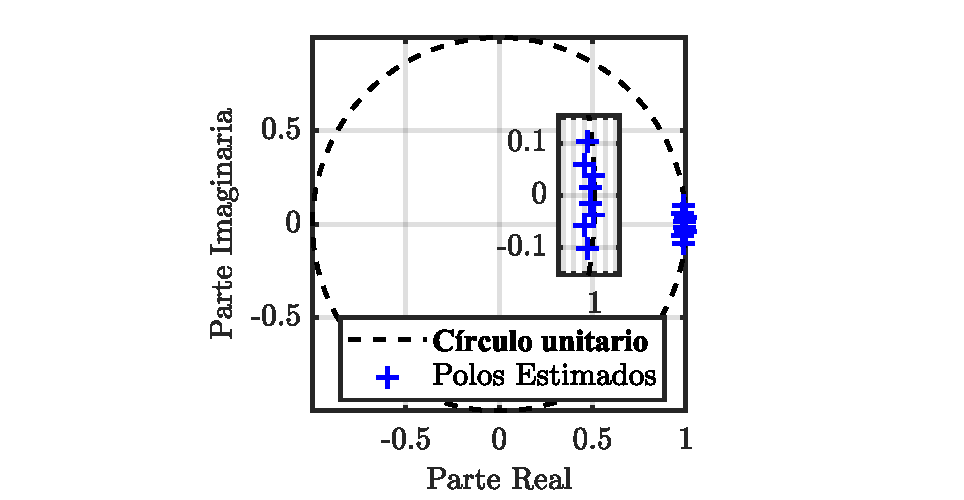
\includegraphics[width=1.05\columnwidth]{Plano Z.pdf} 
    \caption{Ubicación de los polos en el plano Z.}
    \label{fig:plano_z}
\end{figure}


\begin{figure}[htbp]
    \centering
    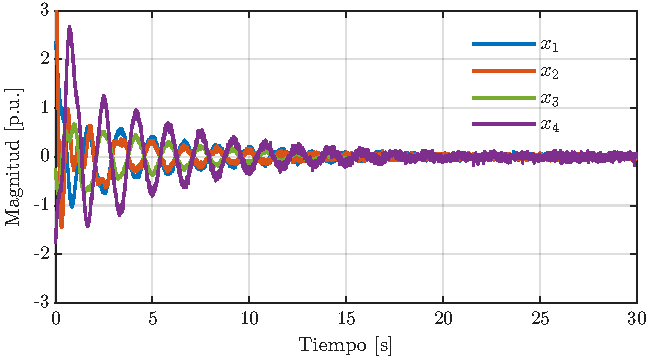
\includegraphics[width=\columnwidth]{Comparacion.pdf}
    \caption{Comparación entre las señales originales  y las señales reconstruidas.}
    \label{fig:comparacion}
\end{figure}


La Fig. \ref{fig:plano_z} muestra la ubicación de las raíces del polinomio de predicción encontrado por el método Multi-TK en el plano Z. Como se observa en la Fig. \ref{fig:plano_z}, los polos correspondientes a los modos oscilatorios de la señal se ubican claramente fuera del círculo unitario. Este resultado es fundamental, ya que confirma que la formulación de predicción hacia atrás, núcleo de la teoría de Tufts-Kumaresan, se ha implementado con éxito. Esta separación geométrica permite distinguir de manera inequívoca los modos reales del sistema de los polos espurios que introduce el ruido, demostrando la robustez teórica del método.

La Tabla~\ref{tab:resultados} presenta los parámetros modales estimados por el algoritmo Multi-TK. Se observa una excelente concordancia con los valores reales, lo que valida la precisión del método.

\begin{table}[htbp]
\caption{Parámetros modales estimados por el algoritmo Multi-TK.}
\label{tab:resultados}
\centering
\begin{tabular}{c|c|c|c|c}
\toprule
Modo &  (\(\lambda = -\delta + j\omega\)) &  (Hz) &  \(\zeta\) (\%) & Descripción \\
\midrule
1 & \(-1.7907 + j5.9690\)  & 0.95 & 28.73 & Local \\
2 & \(-0.8294 + j10.3673\) & 1.65 & 7.97  & Local \\
3 & \(-0.1885 + j3.7699\)  & 0.60 & 4.99  & Inter-área \\
4 & \(-0.7854 + j1.5708\)  & 0.25 & 44.72 & Inter-área \\
\bottomrule
\end{tabular}
\end{table}

\subsubsection{Análisis de Magnitudes y Fases}
Las matrices de magnitudes estimadas \(|a_{i,k}|\) y fases \(\phi_{i,k}\) (en grados) para las cuatro señales se muestran a continuación:

\begin{equation}
\mathbf{M} = 
\begin{bmatrix}
0.50 & 0.20 & 1.00 & 1.00 \\
1.20 & 3.00 & 0.70 & 1.15 \\
0.50 & 0.20 & 0.85 & 0.50 \\
0.75 & 0.20 & 1.95 & 1.25
\end{bmatrix},
\end{equation}

\begin{equation}
\mathbf{\Phi} = 
\begin{bmatrix}
 45.00 & -90.00 &   0.00 &  -0.00 \\
  0.00 &  60.00 &   0.00 & -30.00 \\
 90.00 &  -0.00 & -180.00 &  36.00 \\
-60.00 & -180.00 & -180.00 & -90.00
\end{bmatrix}.
\end{equation}

Cada fila corresponde a una señal (\(i = 1\) a \(4\)) y cada columna a un modo (\(k = 1\) a \(4\)).

\subsubsection{Identificación de Grupos Coherentes en el Modo Inter-área (0.6 Hz)}
El modo 3 (\(f = 0.60\) Hz) es de tipo inter-área. Las fases estimadas para este modo son:

\begin{equation}
\phi_{1,3} = 0^\circ,\quad \phi_{2,3} = 0^\circ,\quad \phi_{3,3} = -180^\circ,\quad \phi_{4,3} = -180^\circ.
\end{equation}

Las señales 1 y 2 presentan una fase de \(0^\circ\), mientras que las señales 3 y 4 presentan una fase de \(-180^\circ\) (equivalente a \(180^\circ\)). Esto indica que los generadores 1 y 2 oscilan en fase entre sí y en completa oposición de fase con los generadores 3 y 4. Por lo tanto, se identifican dos grupos coherentes: \textbf{Grupo A} (señales 1 y 2) y \textbf{Grupo B} (señales 3 y 4). Esta es la firma característica de un modo inter-área, donde dos áreas del sistema oscilan una contra la otra.

Las magnitudes asociadas a este modo (\(|a_{1,3}| = 1.00,\; |a_{2,3}| = 0.70,\; |a_{3,3}| = 0.85,\; |a_{4,3}| = 1.95\)) muestran que la participación es significativa en todas las señales, siendo la señal 4 la de mayor amplitud. Esto confirma que el modo está bien excitado y es globalmente observable.

\subsubsection{Análisis de los Modos Locales}
Los modos 1 y 2 presentan comportamientos locales, como se esperaba de sus frecuencias más altas (0.95 Hz y 1.65 Hz). Por ejemplo, en el modo 1 (0.95 Hz), las fases son \(\phi_{1,1}=45^\circ\), \(\phi_{2,1}=0^\circ\), \(\phi_{3,1}=90^\circ\) y \(\phi_{4,1}=-60^\circ\), sin una agrupación clara en dos bloques definidos, lo que indica que se trata de un modo donde la oscilación se concentra en un generador o en un área pequeña sin una oposición global. 

% --- SECCIÓN IV: CASO DE ESTUDIO II (MODIFICADO) ---
\section{Caso de Estudio II: Sistema IEEE 68-Bus}

Para evaluar el desempeño del método Multi-TK en un entorno de red mas grande y realista, se aplicó el algoritmo al sistema de prueba de 68-bus, el cual consta de 16 generadores divididos en 5 áreas interconectadas (Sistema de New York, sistema de New England y tres áreas vecinas equivalentes). Este sistema es un estándar para el estudio de oscilaciones inter-área debido a su topología extendida y la presencia de modos de baja frecuencia.

El análisis se basa en el procesamiento de datos transitorios (trasn una falla significativa). Esta aproximación permite la identificación de modos para su posterior análisis.


\subsection{Caracterización Profunda de los Modos Identificados}
El algoritmo Multi-TK identificó con éxito los modos críticos que se muestran en \ref{tab:resultados2}, el primer modo corresponde al modo global devido a la formulacion de la matriz de estado como ya se explico, en este caso no es cero, debido a los errores provenientes de las  iteraciones de los flujos de potencia, el modo 2 y 3 presentan caracterisicas inter-áreas, los modos 4 y 5 son locales. A continuación, se discuten los tres modos más relevantes bajo el marco de caracterización propuesto en \cite{ordonez}, que enfatiza la importancia de la "forma del modo" (mode shape) para entender la interacción física.

\begin{table}[htbp]
\caption{Parámetros modales para el Sistema IEEE 68-Bus.}
\label{tab:resultados2}
\centering
\begin{tabular}{c|c|c|c|c}
\toprule
Modo &  (\(\lambda = -\delta + j\omega\)) &  (Hz) &  \(\zeta\) (\%) & Descripción \\
\midrule
1 & \(-0.0010 + j0.0000\)  & 0.000 & 100.00 & Global \\
2 & \(-0.0012 + j0.0403\)  & 0.385 & 3.04  & Local \\
3 & \(-0.0030 + j0.0666\)  & 0.636 & 4.55  & Local\\
4 & \(-0.0044 + j0.0991\)  & 0.946 & 4.46  & Inter-área \\
5 & \(-0.0086 + j0.1297\)  & 1.238 & 6.61  & Inter-área \\
\bottomrule
\end{tabular}
\end{table}

\subsubsection{Modo Inter-área Dominante (0.385 Hz)}
Este es el modo más crítico del sistema IEEE 68-bus, conocido por involucrar la oscilación de todo el sistema de Nueva Inglaterra  y Nueva York contra las áreas externas interconectadas.

\begin{figure}[htbp]
    \centering
    \includegraphics[width=\columnwidth]{ModoInter1.pdf}
    \caption{Vizualización del modo de 0.385 Hz.}
    \label{fig:modo_038}
\end{figure}

Como se observa en la Fig. \ref{fig:modo_038}, existe una coherencia de fase distingible dentro de los grupos. El Grupo 1 (tonos rojos), que incluye los generadores G1 a G13 (NY-NE), oscila en oposición de fase ($~180^\circ$) respecto al Grupo 2 (tonos azules), conformado por G14, G15 y G16. 

Según \cite{roger}, esta estructura modal clara indica las líneas críticas en la transmisión de potencia entre estas áreas. La gran magnitud de participación de los generadores G15 y G16 sugiere que cualquier controlador de amortiguamiento (PSS) debería ubicarse prioritariamente en estas máquinas para ser efectivo.

\subsubsection{Modo Inter-área Secundario (0.636 Hz)}
La Fig. \ref{fig:modo_064} revela un segundo modo inter-área con un comportamiento distinto.

\begin{figure}[htbp]
    \centering
    \includegraphics[width=\columnwidth]{ModoInter2.pdf}
    \caption{Vizualización del modo de 0.636 Hz.}
    \label{fig:modo_064}
\end{figure}

A diferencia del modo de 0.385 Hz, aquí la oscilación está más localizada en la interacción entre el área del sistema de Nueva Inglaterra contra el resto de la red. La amplitud en el área del sistema de Nueva York (G1-G9) es comparativamente mayor pero se observa comportamiento similar en las zonas restantes. Identificar esta diferencia entre modos inter-área es vital, ya que un PSS sintonizado para el modo de 0.385 Hz podría tener poca autoridad sobre este modo de 0.636 Hz.

\subsubsection{Modo Local (0.993 Hz)}
Finalmente, el modo de 0.993 Hz (Fig. \ref{fig:modo_099}) muestra una distribución sin la formación de grandes grupos coherentes, en este caso el modo local pertence al sistema de Nueva York, y las maquinas G4-G7 esatn oscilando en contra de las maquinas G2, G3 y G9. Esto confirma su naturaleza local, donde máquinas individuales oscilan contra la red inmediata, un comportamiento que requiere sintonización local de controladores.

\begin{figure}[htbp]
    \centering
    \includegraphics[width=\columnwidth]{ModoLocal1.pdf}
    \caption{Vizualización del modo local de 0.993 Hz.}
    \label{fig:modo_099}
\end{figure}

\section{Validación }

La Fig. \ref{fig:datos_vs_mtk} demuestra que el modelo lineal de bajo orden obtenido por Multi-TK captura con precisión la dinámica compleja de la señal original. La coincidencia en fase y amplitud confirma que los modos extraídos (0.38 Hz, 0.64 Hz, etc.) son los verdaderos modos físicos que gobiernan la dinámica del sistema Nueva York - Nueva Inglaterra. 

\begin{figure}[htbp]
    \centering
    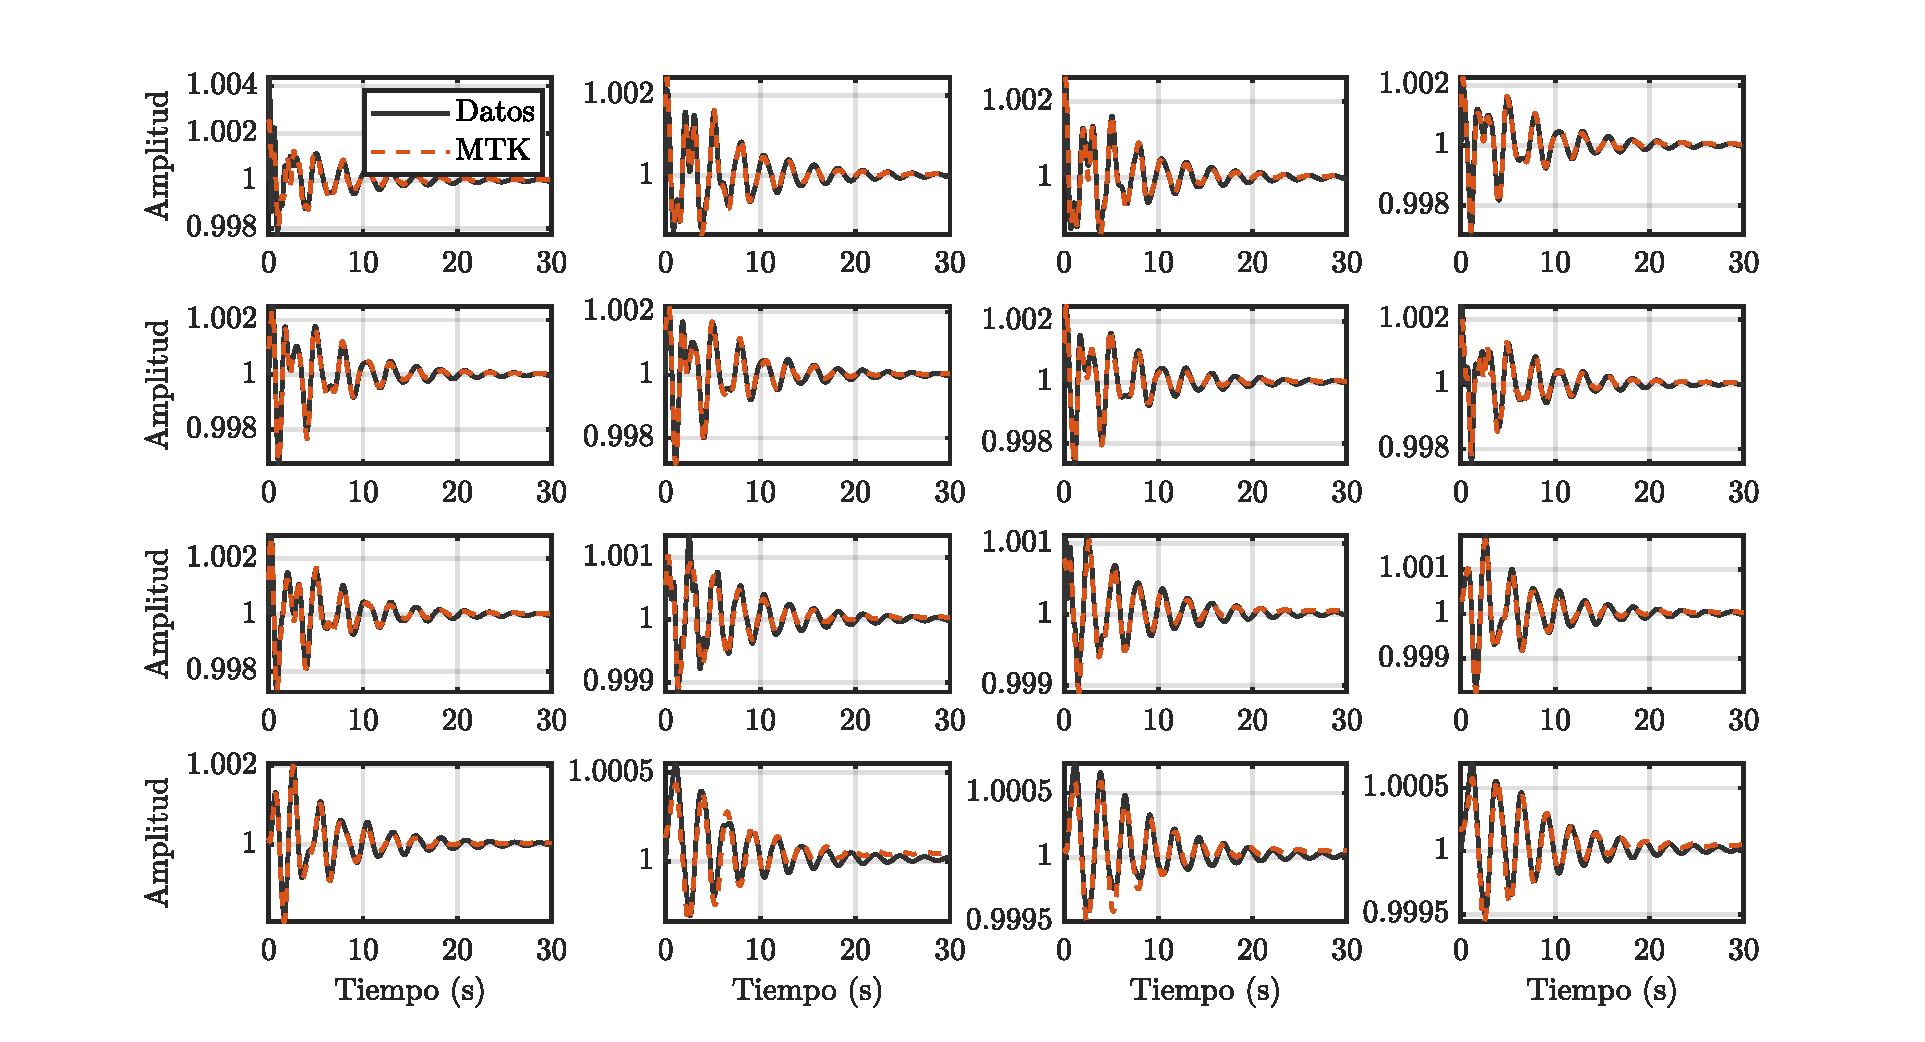
\includegraphics[width=\columnwidth]{DATOS_vs_SVG.pdf}
    \caption{Validación temporal: Superposición de la señal medida (negro) y la señal reconstruida por Multi-TK (rojo).}
    \label{fig:datos_vs_mtk}
\end{figure}


\subsection{Análisis espectral}

La Fig. \ref{fig:fft_39bus} muestra el espectro (FFT) de la velocidad de los generadores. Se evidencian picos de energía significativos en la banda de 0.2 a 0.8 Hz, característicos de interacciones entre grandes áreas geográficas, y picos superiores a 0.9 Hz asociados a modos locales, lo que valida los modos estimados por el algoritmo Multi-TK.

\begin{figure}[htbp]
    \centering
    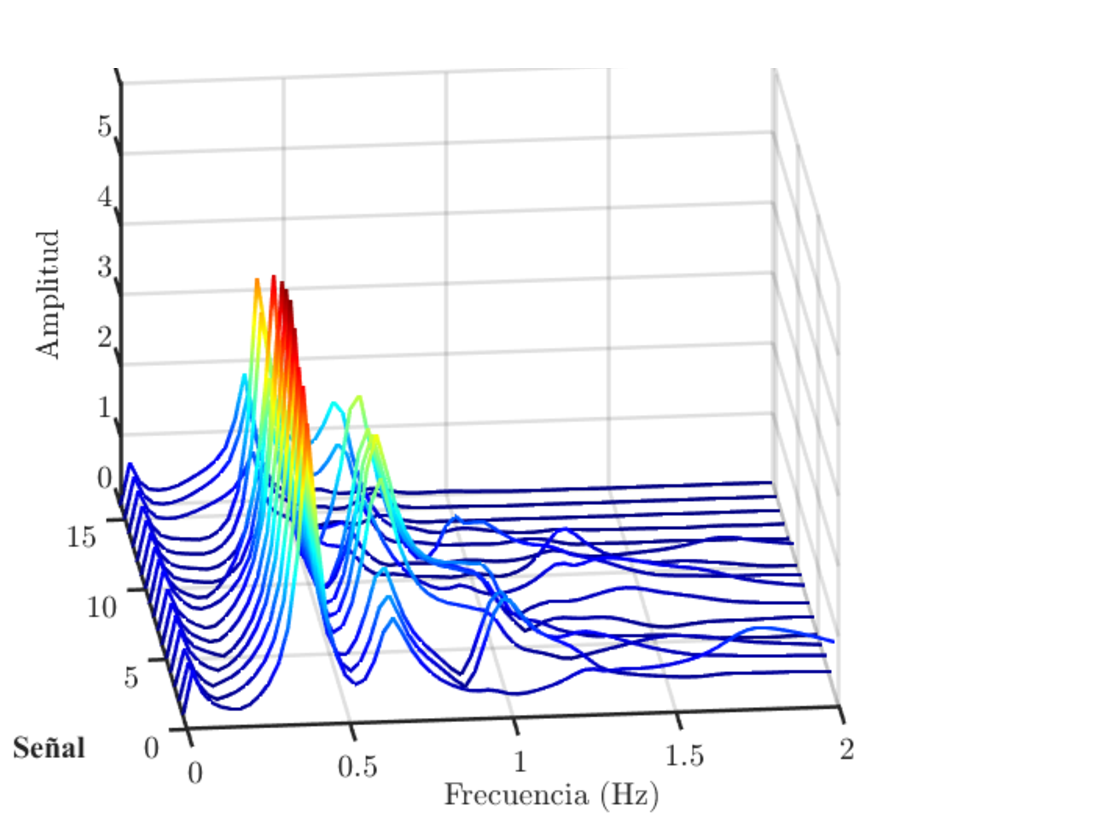
\includegraphics[width=\columnwidth]{FFT_V1.pdf}
    \caption{Espectro de frecuencia (FFT) de los 16 generadores del sistema IEEE 68-Bus. Nótese la energía dominante en frecuencias < 0.7 Hz.}
    \label{fig:fft_39bus}
\end{figure}

% --- SECCIÓN V: CONCLUSIONES ---
\section{Conclusiones}

En este trabajo se ha desarrollado y validado una expansión multiseñal del algoritmo Tufts-Kumaresan (Multi-TK), diseñada específicamente para el monitoreo de la estabilidad dinámica en sistemas eléctricos de potencia modernos. A diferencia de los enfoques convencionales que analizan señales de forma aislada, la formulación propuesta integra de manera coherente los flujos de datos de los Sistemas de Medición de Área Amplia (WAMS). La implementación de un modelo de predicción hacia atrás, fortalecido por la Descomposición en Valores Singulares (SVD) truncada, permitió una separación efectiva entre los modos físicos del sistema y los componentes no deseadas, asegurando una identificación modal precisa incluso en condiciones transitorias complejas.

Los resultados obtenidos mediante el análisis del sistema de 68 buses confirman que el método es capaz de capturar la dinámica global de la red con una fidelidad decente. La caracterización profunda de las "formas de modo" (mode shapes) facilitó la distinción clara entre oscilaciones locales y modos inter-área críticos, como el observado a 0.385 Hz que involucra la interacción entre las áreas de Nueva York y Nueva Inglaterra. Esta capacidad de identificar no solo la frecuencia y el amortiguamiento, sino también la coherencia de fase y el nivel de participación de cada generador, constituye una herramienta de alto valor estratégico para la ubicación y sintonización de Estabilizadores de Sistemas de Potencia (PSS), optimizando así las acciones de control ante posibles contingencias.

En conclusión, el algoritmo Multi-TK ofrece un balance óptimo entre eficiencia computacional y robustez analítica, superando las limitaciones de consistencia de los métodos paramétricos tradicionales. Las validaciones tanto en el dominio del tiempo como en el de la frecuencia demuestran que el modelo lineal de bajo orden extraído representa fielmente los fenómenos físicos subyacentes. Como líneas de investigación futuras, se contempla la evolución de este marco hacia una implementación recursiva y adaptativa que permita el seguimiento de modos en tiempo real bajo condiciones de operación altamente cambiantes. Asimismo, se explorará la integración de técnicas avanzadas de pre-filtrado para mantener el desempeño del algoritmo ante pérdida de datos en las PMU.

% --- REFERENCIAS ---
\begin{thebibliography}{99}

\bibitem{kundur}
P.~Kundur, \emph{Power System Stability and Control}, New York, NY, USA: 1st~ed. McGraw-Hill, 1994.


\bibitem{roger}
G. Rogers, R. Elliott, D. Trudnowski, F. Wilches-Bernal, D. Osipov, J. Chow, \emph{Power System Oscillations: An Introduction to Oscillation Analysis and Control}, New York, NY, USA: 2nd~ed. Springer, 2025.


\bibitem{tufts}
R. Kumaresan y D. W. Tufts, \emph{Estimating the parameters of exponentially damped sinusoids and pole-zero modeling in noise}, IEEE Transactions on Acoustics, Speech, and Signal Processing, vol.~30, no.~6, pp.~833-840, Dec. 1982, doi: 10.1109/TASSP.1982.1163974.


\bibitem{moghdam}
Alizadeh Moghdam, M., Noroozian, R., y Jalilzadeh, S. \emph{Improving the accuracy and the estimation time of inter-area modes in power system based on Tufts-Kumaresan algorithm}, International Journal of Modelling and Simulation, vol. 44, no.~3, pp.~126-135, 2024, doi: 10.1080/02286203.2022.2161443 


\bibitem{Trudnowski}
D. J. Trudnowski, J. Follum, R. T. Elliott, D. A. Schoenwald y J. W. Pierre \emph{Characterizing the Oscillatory Properties of Bulk Electric Systems}, IEEE Access, vol. 13, pp. 32883-32900, 2025, doi: 10.1109/ACCESS.2025.3543457.


\bibitem{ordonez}
J. Ramos, R. Jimenez y E. Barocio, \emph{Visualization of interarea oscillations using an extended subspace identification technique}, North American Power Symposium (NAPS), Manhattan, KS, USA,pp. 1-6, 2013, doi: 10.1109/NAPS.2013.6666931.


\end{thebibliography}

\end{document}